\chapter{針對不同使用情境進行最佳化}
\label{chp:5}

\begin{figure}[htpb]
    \centering
    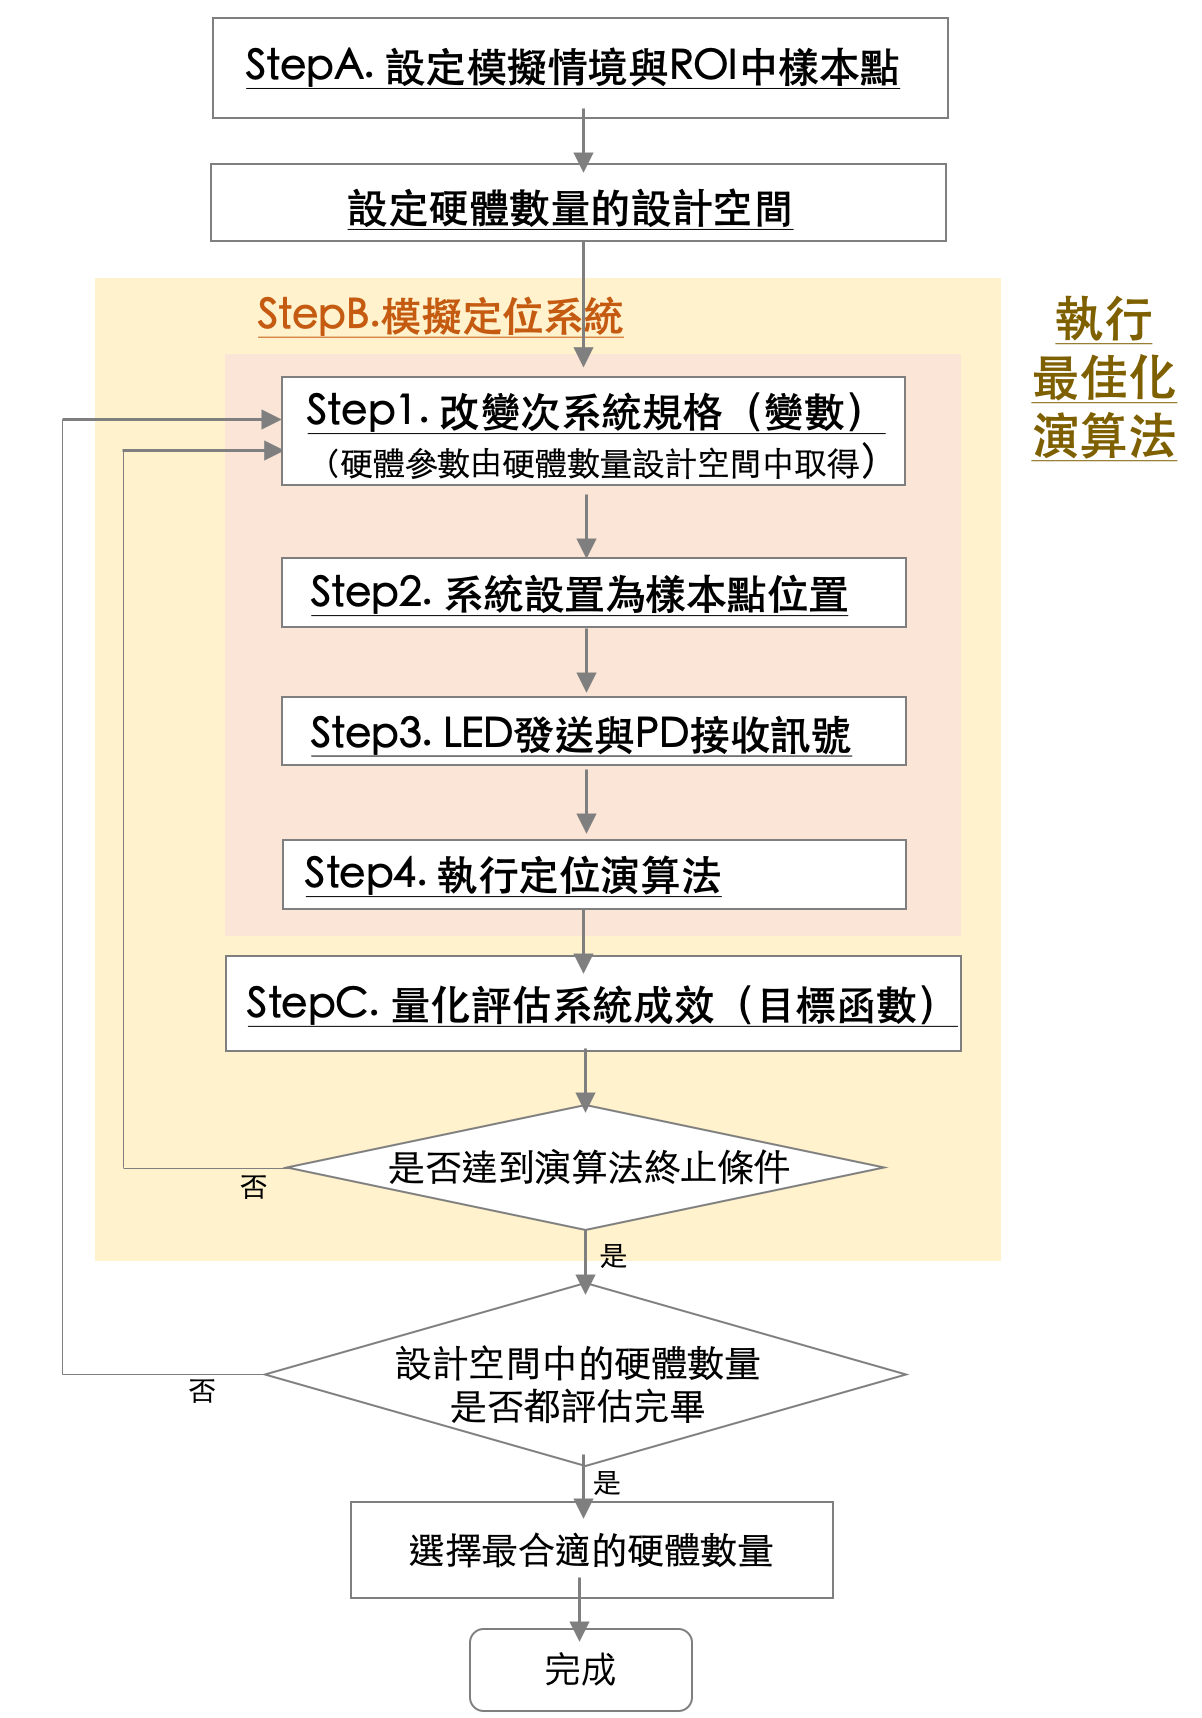
\includegraphics[width=10cm]{ch5pic/optimize_flow.png}
    \caption{最佳化流程圖}
    \label{pic:optimize_flow}
\end{figure}

我們於第四章中,討論了不同次系統規格的變數對硬體成效的影響,然而在第四章中為了方便分析,我們限制硬體指向使變數只剩下LED與PD的硬體天頂角;在分析上,各參數的影響也僅透過固定其他參數來作分析。因此,當我們想要針對特定使用情境,得到最好的次系統規格,則需要透過最佳化問題來解答。本章節於依序於\ref{chp:optimize}章定義最佳化問題,並於章中針對\ref{chp:scenario}章中室內定位的例子,於\ref{chp:optimize_case}章給出最佳系統設計,最後於\ref{chp:5_conclu}中進行總結。




因此,本章節的最佳化問題中,最佳化變數包含Step1.決定次系統規格中的:朗博次方$Mp,M\ell$、各硬體指向$^{P}\boldsymbol{V}_p,^{L}\boldsymbol{V}_l$與硬體數量$P,L$,而其中每個硬體皆有硬體指向需要定義,LED在指向總共會有$2L$個自由度、PD則有$2P$個指向自由度。因此最佳化變數的變數總量,又會根據最佳化本身而改變,使得最佳化難度高。因此,為了簡化這個變數數量與變數本身相關的問題,我們將硬體數量獨立出來迭代執行評估,參考流程圖\ref{pic:optimize_flow},與系統評估流程圖\ref{pic:evaluate_flow}相似,由StepA.設定使用情境與ROI中樣本點開始,再設定LED與PD硬體數量的設計空間,接著於StepB.中決定次系統規格並以模擬呈現系統定位流程,最後於StepC.量化系統成效。其中,針對朗博次方與指向的最佳化問題,我們使用基因演算法(Genetic Algorithm,以下簡稱GA)求解,得到該硬體總數$L$與$P$的系統規格中,朗博次方與指向的最佳解後,透過迭代改變硬體數量,最後再人為評估最合適的硬體數量,作為系統最佳解。

% 硬體數量確定後,而,我們可以得到不同硬體數量對應的最佳設計,以及該設計的目標函數。擁有這些資訊,即可透過人類決策者介入選擇,在系統表現以及硬體成本中進行取捨。

% 最佳化流程可藉由對系統評估流程圖\ref{pic:evaluate_flow}修改,呈現於圖\ref{pic:optimize_flow}中。

% 流程其中StepB.中的Step1.決定次系統規格,即為最佳化變數,而StepC.量化系統成效則為目標函數。與系統評估流程差異最大的部分為StepA.與StepB.之間出現的設定硬體數量設計空間,並透過迭代對硬體數量設計空間中的每個設計點進行其他次系統規格參數的最佳化。將硬體數量獨立出來的原因是為了避免最佳化問題過於複雜,詳細可參考\ref{chp:optimize_variable}章。

% 接著與系統評估流程不同,我們將


以下章節依序由\ref{chp:objective}章中介紹目標函數,於\ref{chp:optimize_variable}章中介紹最佳化變數,而\ref{chp:optimize_case}章中則針對情境進行系統最佳化。

\section{最佳化問題}
\label{chp:optimize}
    \subsection{目標函數}
    \label{chp:objective}

    我們的最佳化目標,是希望使系統表現更好,而評估方式可以參考\ref{chp:evaluate_method}章所述,目標是讓在容許範圍內的樣本點比例越高越好。因此,在硬體總數設定為$P,L$的情況下,最佳化目標函數$f$呈現於式\ref{eqn:objective}

    \begin{equation}
        \label{eqn:objective}
        \begin{aligned}
        \underset{^{P}\boldsymbol{V}_p, ^{L}\boldsymbol{V}_l,Ml,Mp}{\operatorname{minimize}} 
        \quad f = 
        \frac{\sum_{i=1}^{K}F(k)}{K}  \\
        \text{Where }F(k)=
        \begin{cases}
            _{k}e<To&,1\\
            else&,0
        \end{cases}
        \end{aligned}
    \end{equation}

    \begin{align*} \text{where }
        &p=1,2,...,P\\&l=1,2,...,L
    \end{align*}


    \subsection{最佳化變數}
    \label{chp:optimize_variable}

    最佳化變數的部分,包含朗博次方$Mp,M\ell$、硬體指向$^{P}\boldsymbol{V}_p,^{L}\boldsymbol{V}_l$與硬體數量$P,L$,而其中每個硬體皆有朗博次方與硬體指向需要定義,因此最佳化的變數量又會根據硬體數量而改變,變數總數為$2+2\times(L+P)$。


    \begin{figure}[h!]
        \centering
        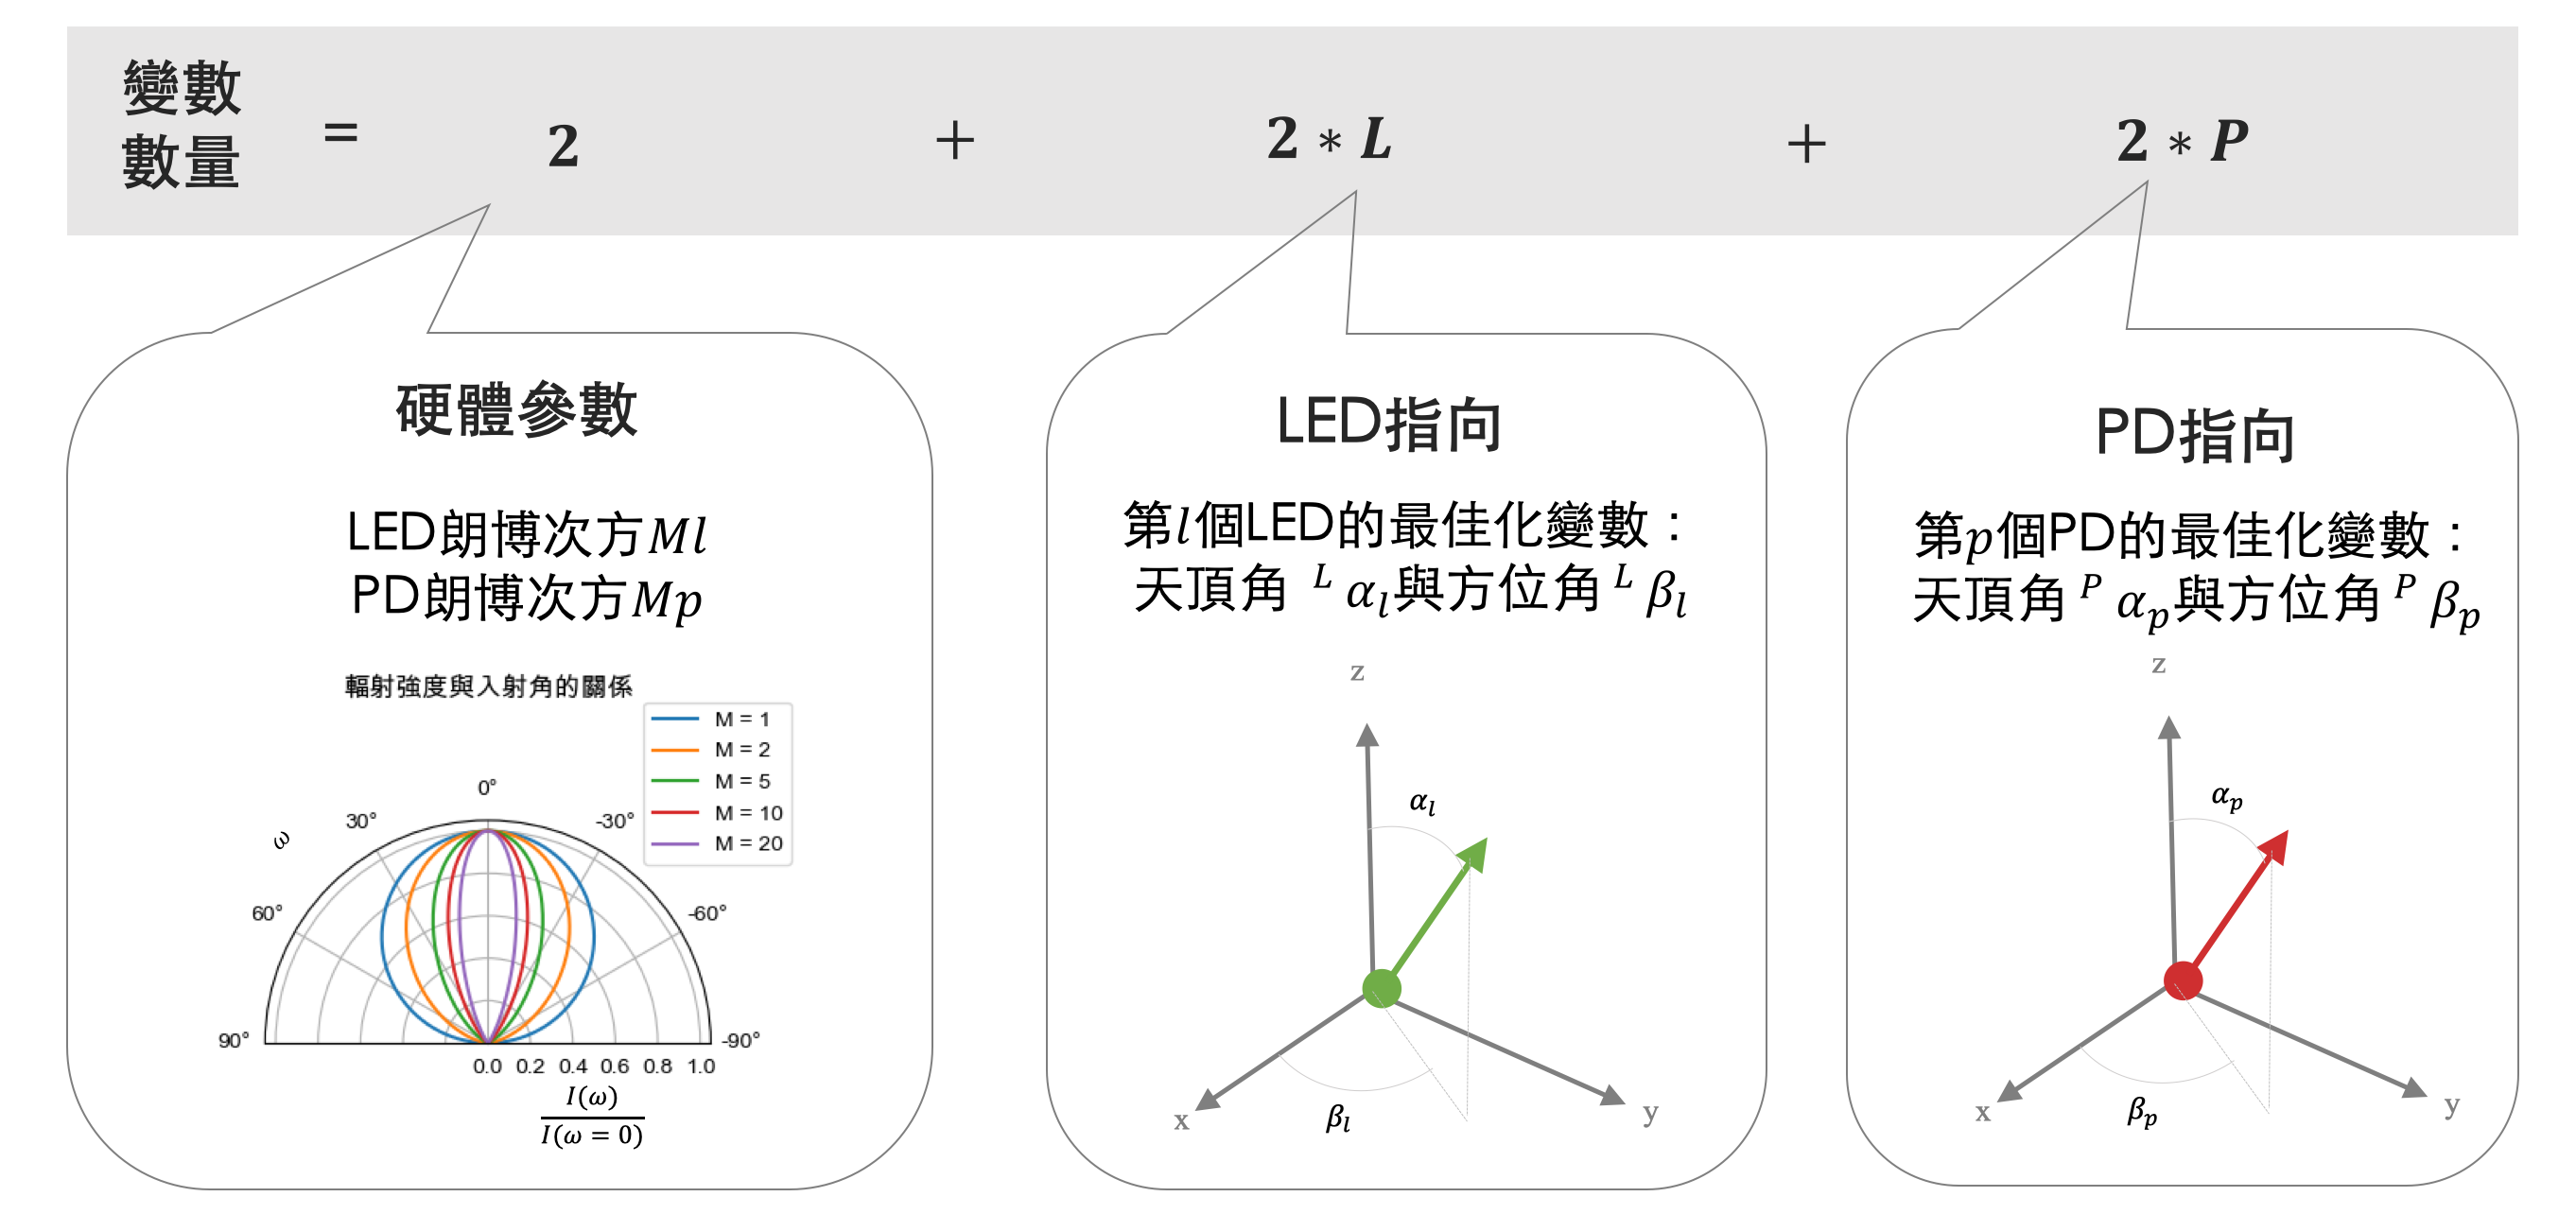
\includegraphics[width=15cm]{ch5pic/optimize_variable.png}
        \caption{最佳化變數}
        \label{pic:optimize_variable}
    \end{figure}



% --------------------------------------
\section{案例}
\label{chp:optimize_case}

    \subsection{室內空間的案例}

    我們最佳化的目標情境參考\ref{chp:scenario}章,為一包含平移樣本與旋轉樣本的的室內空間,而以下圖\ref{pic:opt_result}呈現硬體數量分別為$P=L=5$以及$P=L=10$時,朗博次方與硬體指向的最佳化結果。

    \begin{figure}[htpb]
        \centering
        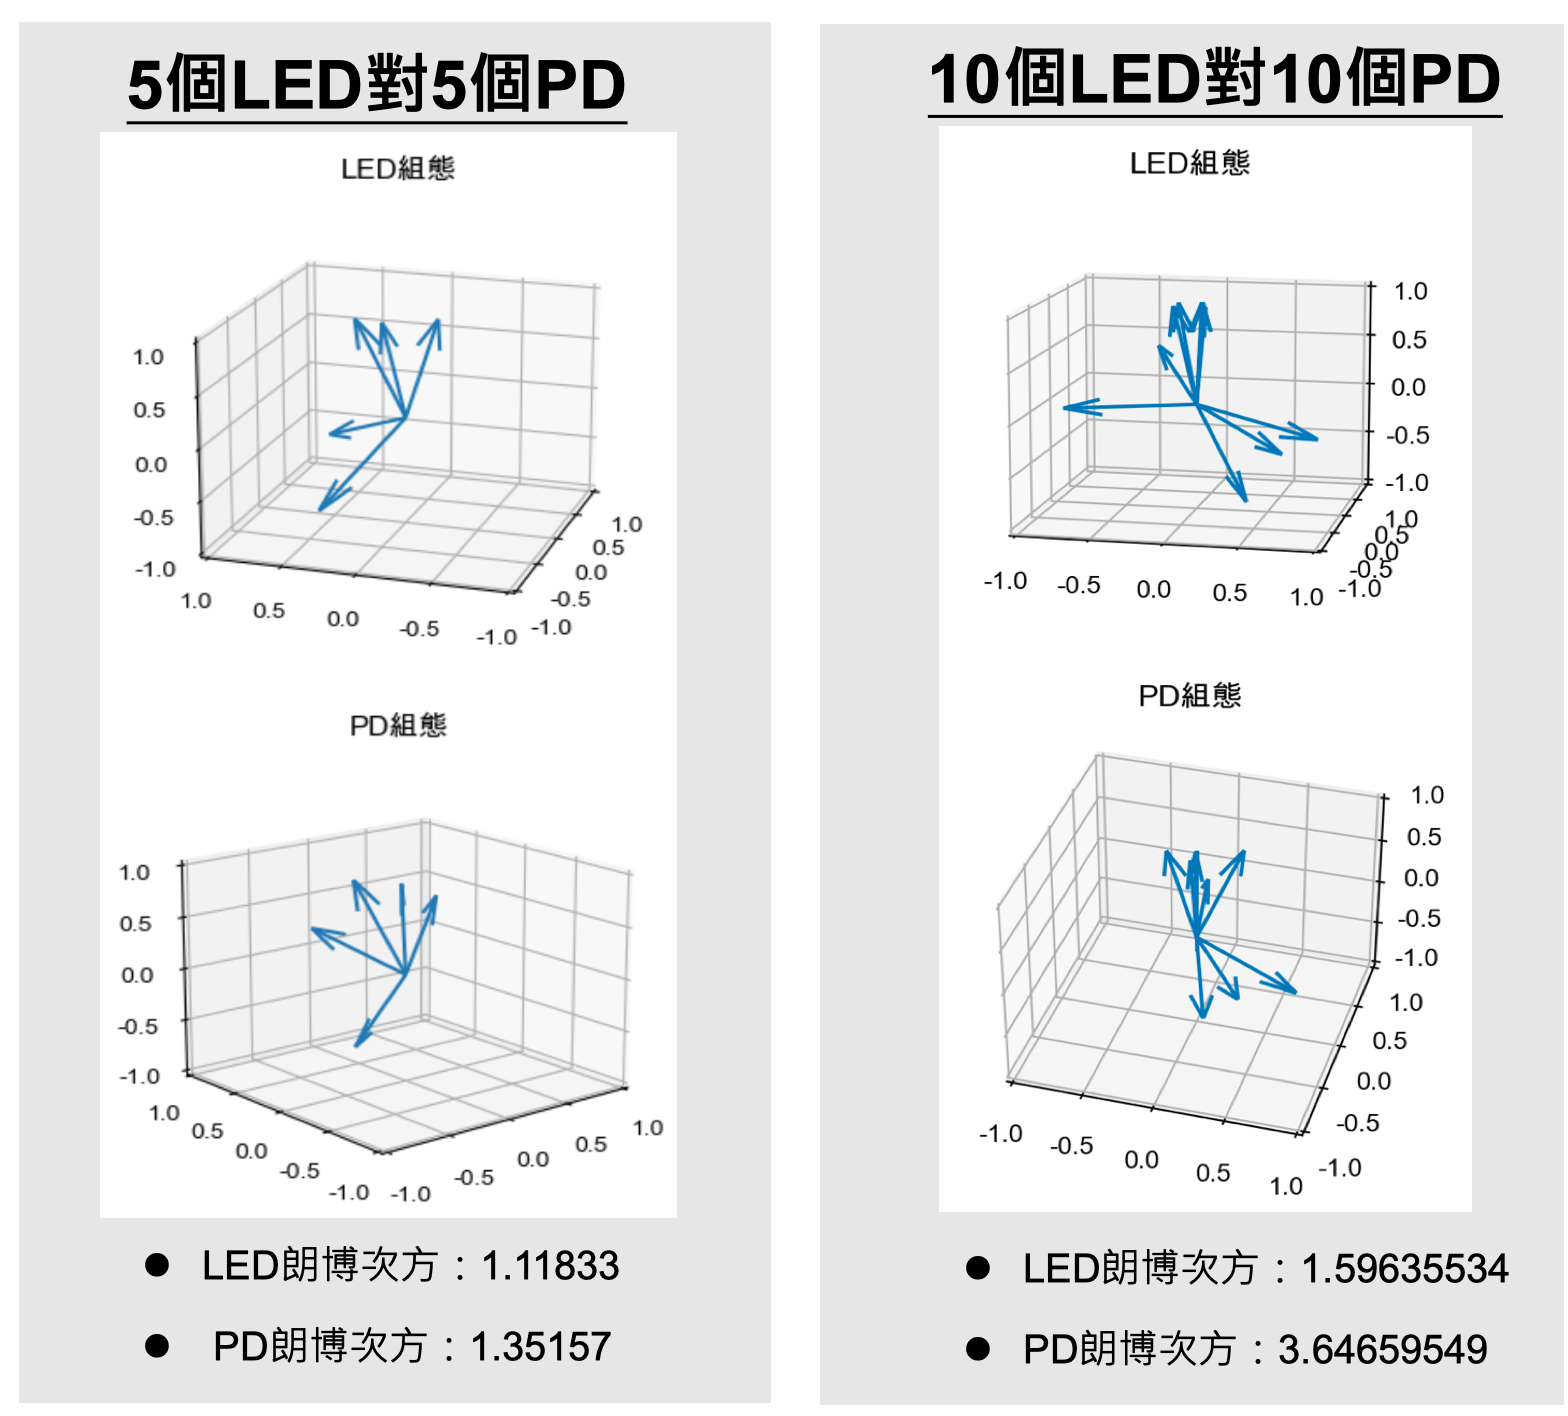
\includegraphics[width=15cm]{ch5pic/opt_result.png}
        \caption{最佳化結果}
        \label{pic:opt_result}
    \end{figure}

    觀察這兩個系統設計的差別,在硬體數量少的時候,為了讓空間中的最多個樣本點可讀到訊號,因此朗博次方較小,捨棄了對出入射角敏感度。

    % \subsection{以目標物為中心的案例}


% --------------------------------------
\section{結論}
\label{chp:5_conclu}

本章節提出一流程,針對不同使用情境,進行朗博次方$Mp,M\ell$、硬體指向$^{P}\boldsymbol{V}_p,^{L}\boldsymbol{V}_l$與硬體數量$P,L$的最佳化。透過設定不同的情境、不同的參數,我們可以得到最適合的朗博次方與硬體擺設設計,也知道不同硬體數量的表現。有了最佳化後的結果,我們可以參考最佳朗博次方,於市售硬體中挑選接近的硬體,並再以\ref{chp:simulation}章中介紹的模擬方式,對該次系統硬體規格的系統進行定位成效評估,確認次系統設計符合需求,再進行硬體的購買以及硬體系統的搭建。透過軟體的模擬與最佳化,我們可以減少硬體系統重複測試的麻煩。













